\section{Lancement de l'application}

\begin{figure}[h]
\centering
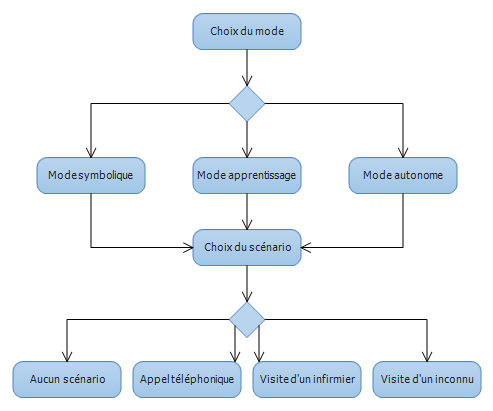
\includegraphics[width=1\textwidth]{4-Conception/img/diagActivite.png}
\caption{ Diagramme d'activité}
\end{figure}

Au lancement du logiciel, l'utilisateur peut personnaliser la simulation à travers plusieurs options.

Tout d'abord, il peut choisir un mode d'apprentissage. Ces modes apportent de l'autonomie ou donnent des directions à l'utilisateur en lui donnant des indicateurs visuels sur ce qu'il peut faire. Voici les différents modes :
\begin{itemize}
\item Symbolique ;
\item Assisté ;
\item Autonome.
\end{itemize}

\vspace{\parskip}

De plus, il est possible de jouer un scénario, pour forcer l'utilisateur à faire certains choix et interagir avec certains objets. Voici les différents scénarios :
\begin{itemize}
\item Appel téléphonique normal ;
\item Appel \textit{via} l'interphone d'une personne venant fréquemment (un infirmier par exemple) ;
\item Appel \textit{via} l'interphone concernant une visite inattendue.
\end{itemize}

\vspace{\parskip}

Ces différents choix seront gérés par des scripts C\# de Unity, et plus précisement par le GameManager, décrit dans la section \ref{modelisation} de ce rapport.

